\documentclass[notes,11pt, aspectratio=169, usenames, dvipsnames]{beamer}

\usepackage{pgfpages}
% These slides also contain speaker notes. You can print just the slides,
% just the notes, or both, depending on the setting below. Comment out the want
% you want.
%\setbeameroption{hide notes} % Only slide
%\setbeameroption{show only notes} % Only notes
\setbeameroption{show notes on second screen} % Both

%\usepackage{helvet}
%\usepackage[default]{lato}
\usepackage{bookman}
\usepackage{array}

%%% TIKZ STUFF
\usepackage{tikz}
\usetikzlibrary{positioning}
\usetikzlibrary{snakes}
\usetikzlibrary{calc}
\usetikzlibrary{arrows}
\usetikzlibrary{decorations}
%\usetikzlibrary{decorations.markings}
%\usetikzlibrary{shapes.misc}
\usetikzlibrary{matrix,shapes,arrows,fit, arrows.meta, tikzmark}
\tikzset{  
	-Latex,
	auto,
	node distance = 1 cm and 1 cm,
	semithick,
	every picture/.style={remember picture,baseline},
	every node/.style={anchor=base,align=center,outer sep=1.5pt},
	every path/.style={thick},
	state/.style ={ellipse, draw, minimum width = 0.7 cm},
	point/.style = {circle, draw, inner sep=0.04cm,fill,node contents={}},
	bidirected/.style={Latex-Latex,dashed},
	latent/.style={dashed},
	el/.style = {inner sep=2pt, align=left, sloped}
}
\newcommand\marktopleft[1]{%
	\tikz[overlay,remember picture] 
	\node (marker-#1-a) at (-.3em,.3em) {};%
}
\newcommand\markbottomright[2]{%
	\tikz[overlay,remember picture] 
	\node (marker-#1-b) at (0em,0em) {};%
}
\tikzstyle{every picture}+=[remember picture] 
\tikzstyle{mybox} =[draw=black, very thick, rectangle, inner sep=10pt, inner ysep=20pt]
\tikzstyle{fancytitle} =[draw=black,fill=red, text=white]
%%%% END TIKZ STUFF

\usepackage{verbatim}
\setbeamertemplate{note page}{\pagecolor{yellow!5}\insertnote}
\usepackage{amsmath}
\usepackage{xfrac}
\usepackage{mathpazo}
\usepackage{hyperref}
\usepackage{lipsum}
\usepackage{multimedia}
\usepackage{animate}
\usepackage{graphicx}
\usepackage{multirow}
\usepackage{graphicx}
\usepackage{dcolumn}
\usepackage{bbm}
\newcolumntype{d}[0]{D{.}{.}{5}}
\usepackage{makecell}


% Tabular line breaks
\usepackage{tabularx}
\renewcommand\theadalign{bc}
\renewcommand\theadfont{\bfseries}
\renewcommand\theadgape{\Gape[4pt]}
\renewcommand\cellgape{\Gape[4pt]}

\usepackage{changepage}
\usepackage{appendixnumberbeamer}
\newcommand{\beginbackup}{
   \newcounter{framenumbervorappendix}
   \setcounter{framenumbervorappendix}{\value{framenumber}}
   \setbeamertemplate{footline}
   {
     \leavevmode%
     \hline
     box{%
       \begin{beamercolorbox}[wd=\paperwidth,ht=2.25ex,dp=1ex,right]{footlinecolor}%
%         \insertframenumber  \hspace*{2ex} 
       \end{beamercolorbox}}%
     \vskip0pt%
   }
 }
\newcommand{\backupend}{
   \addtocounter{framenumbervorappendix}{-\value{framenumber}}
   \addtocounter{framenumber}{\value{framenumbervorappendix}} 
}

% Math commands
\newcommand{\vect}[1]{\boldsymbol{#1}}
\newcommand*{\Scale}[2][4]{\scalebox{#1}{\ensuremath{#2}}}
\newcommand\independent{\protect\mathpalette{\protect\independenT}{\perp}}
\def\independenT#1#2{\mathrel{\rlap{$#1#2$}\mkern2mu{#1#2}}}

% If you keep your figures in a separate directory, set the path
% to that directory here
\usepackage{graphicx}
\graphicspath{{figures/}}
\usepackage[space]{grffile}
\usepackage{booktabs}

% These are my colors -- there are many like them, but these ones are mine.
\usepackage{xcolor}
\definecolor{cream}{HTML}{E1DAAE}
\definecolor{orange}{HTML}{FF934F}
\definecolor{red}{HTML}{CC2D35}
\definecolor{blue}{HTML}{058ED9}
\definecolor{grey}{HTML}{848FA2}
\definecolor{midnight}{HTML}{2D3142}

\hypersetup{	
  colorlinks=true,
  citecolor = {blue},
  linkbordercolor = {white},
  linkcolor = {blue}
}


%% I use a creamy off white for my background
\definecolor{LightBackground}{RGB}{255,253,218}

%% Uncomment this if you want to change the background color to something else
%\setbeamercolor{background canvas}{bg=LightBackground}

%% Change the bg color to adjust your transition slide background color!
\newenvironment{transitionframe}{
  \setbeamercolor{background canvas}{bg=midnight}
  \begin{frame}}{
    \end{frame}
}

%% Remember to change these if you use the DarkBackground
\setbeamercolor{frametitle}{fg=red}
\setbeamercolor{title}{fg=black}
\setbeamertemplate{footline}[frame number]
\setbeamertemplate{navigation symbols}{} 
\setbeamertemplate{itemize items}{-}
\setbeamercolor{itemize item}{fg=midnight}
\setbeamercolor{itemize subitem}{fg=midnight}
\setbeamercolor{enumerate item}{fg=midnight}
\setbeamercolor{enumerate subitem}{fg=midhgt}
\setbeamercolor{button}{bg=cream,fg=midnight,}



% If you like road maps, rather than having clutter at the top, have a roadmap show up at the end of each section 
% (and after your introduction)
% Uncomment this is if you want the roadmap!
% \AtBeginSection[]
% {
%    \begin{transitionframe}
%        \frametitle{Roadmap of Talk}
%        \tableofcontents[currentsection]
%    \end{transitionframe}
% }
\setbeamercolor{section in toc}{fg=blue}
\setbeamercolor{subsection in toc}{fg=orange}
\setbeamersize{text margin left=1em,text margin right=1em} 

\newenvironment{wideitemize}{\itemize\addtolength{\itemsep}{10pt}}{\enditemize}

\usepackage{environ}
\NewEnviron{videoframe}[1]{
  \begin{frame}
    \vspace{-8pt}
    \begin{columns}[onlytextwidth, T] % align columns
      \begin{column}{.58\textwidth}
        \begin{minipage}[t][\textheight][t]
          {\dimexpr\textwidth}
          \vspace{8pt}
          \hspace{4pt} {\Large \sc \textcolor{red}{#1}}
          \vspace{8pt}
          
          \BODY
        \end{minipage}
      \end{column}%
      \hfill%
      \begin{column}{.42\textwidth}
        \colorbox{orange!20}{\begin{minipage}[t][1.2\textheight][t]
            {\dimexpr\textwidth}
            Face goes here
          \end{minipage}}
      \end{column}%
    \end{columns}
  \end{frame}
}

% If you reference citations and want a bibliography add the .bib here, alter settings, and
% uncomment the \printbibliography at the end
\usepackage[backend=biber, natbib, style=authoryear-comp, citestyle=numeric-comp]{biblatex}
\usepackage{keyval,ifthen}
\usepackage{csquotes}
\addbibresource{causal_inference.bib}

%%%%%%%%%%%%%%%%%%%%%%%%%%%%%%%%%%%%
%%%                              %%%
%%% Start of presentation slides %%%
%%%                              %%%
%%%%%%%%%%%%%%%%%%%%%%%%%%%%%%%%%%%%

\title[]{\textcolor{red}{A (Brief) Introduction to Causal Inference}}
\author[EAJ]{}
\institute[UMDCP]{\small{\begin{tabular}{c c c}
\multicolumn{3}{c}{Evan A. Jones} \\
\multicolumn{3}{c}{University of Maryland -- College Park}

%Author A &&  Author B  \\
%Somewhere Fancy && Somewhere Fancy \\

%Author C && Author D   \\
%\multicolumn{3}{c}{Somewhere Fancy} \\
\end{tabular}}}

\date{\today}


\begin{document}

% Title Slide
\begin{frame}
\maketitle
  \centering Prepared for GVPT's GSA Method Workshop, Spring 2021.
\end{frame}

% INTRO
\begin{frame}{The "Why?" and "What If?" Questions}
	\begin{columns}[T] % align columns
		\begin{column}{.58\textwidth}
			\begin{wideitemize}
				\item[-]<1-> Understanding the world around us is an inherently human endeavor
				\item[-]<2-> Human children explore the world as scientists do \citep{Gopnik2012, BuchsbaumEtal2012}: 
					\begin{itemize}
						\item[-] Asking questions
						\item[-] Forming hypotheses
						\item[-] Testing hypotheses via interventions \citep{GopnikEtal2004}
					\end{itemize}
				\item[-]<3-> By adulthood, we have fairly solid causal intuition about the physical world
			\end{wideitemize}
		\end{column}%
		\hfill%
		\begin{column}{.38\textwidth}
			\makebox[\linewidth][c]{
				\only<2->{\resizebox{\linewidth}{!}{
					
\includegraphics{but_why.jpg}
				}}
			}
		\end{column}%
	\end{columns}
\note[itemize]{
	\item{May not know causal mechanics of physical world down to \textit{functional} form}
	\item{For instance, many adult may not know the Gas laws PV=nRT, but they have a correct, intuitive---or high-level---understanding of the these relationships just based on playing with balloons or filling your bike tires as a kid}
}
\end{frame}



\begin{frame}{The "Why?" and "What If?" Questions}
\begin{columns}[T] % align columns
\begin{column}{.58\textwidth}
  \begin{wideitemize}
    \item[-]<1-> As researchers, we fit regressions all the time and interpret coefficients
    \item[-]<2-> Take the following, for instance :
    $$
    Y = \alpha + \beta x + \theta z + \epsilon 
    $$
    
    \item[-]<3-> When can we interpret $\beta$ as a causal effect?
%    \item Read \emph{\textcolor{blue}{\href{https://www.amazon.com/Better-Presentations-Guide-Scholars-Researchers/dp/0231175213/}{Jon Schwabish's ``Better Presentations''}}}
  \end{wideitemize}
\end{column}%
\hfill%
\begin{column}{.38\textwidth}
  \makebox[\linewidth][c]{
    \only<3->{\resizebox{\linewidth}{!}{
      \animategraphics[autoplay, loop, height=5cm]{1}{figures/chin_scratch_}{0}{18}
    }}
  }
\end{column}%
\end{columns}
\note[itemize]{
	\item{As researchers, we go a step further. Seek to precisely uncover low-level relationships}
	\item{Qualitative researchers also perform causal inference}
	\item{Rather than uncovering functional forms or quantifying effects, seek out entire causal mechanisms or "configurations" of variables}
	\item{So much of what we learn about interpreting regressions through telegraphic readings of the political science literature is simply wrong}
	\item{Not a criticism of previous generations of scholars, causal inference simply not taught in most departments until recently}
	\item{Moreover, causal inference still rarely taught in \textit{statistics departments}}
}
\end{frame}

\begin{frame}{The "Why?" and "What If?" Questions}
	\begin{center}
		{ \Huge What is causality?}
	\end{center}
\note[itemize]{
	\item{\textcolor{blue}{Ask audience to answer this question?}}
	\item{What distinguishes description and prediction from causal inference?}
	\item{How can we move beyond observation, description, and prediction and towards answering causal and counterfactual questions?}
	\item{This talk won't give you every tool you need to perform causal inference in your own project from start to finish}
	\item{Field is much too large for that}
	\item{Hope is to provide you with the philosophical and logical tool kit to engage this literature on your own, and prepare you for presentations to come}
	\item{Relay how I first jumped into this literature, and why starting from "30,000" feet would have been better}
}
\end{frame}

\begin{frame}{Outline}
	\begin{wideitemize}
		\item Logic of Causal Inference
		\item Experiments vs the World
		\item Potential Outcomes vs Structural Causal Models
	\end{wideitemize}
\end{frame}

\section{Logic of Causal Inference}
\begin{transitionframe}
	\begin{center}
		{ \Huge \textcolor{blue}{Logic of Causal Inference}}
	\end{center}
\end{transitionframe}

\begin{frame}{Beyond Description}
	\begin{wideitemize}
		\item<1-> Causal explanations are "more than mere descriptions \ldots of the observed data" \citep[p. 3]{BarenboimEtal2020}
		\item<2-> Break down phenomena into constituent parts and define how parts interact to produce emergent behavior (\textcolor{blue}{\emph{data-generating process}) }\citep{Simon1953}
		\item<3-> Once uncovered, causal mechanisms are powerful
	\end{wideitemize}
\note[itemize]{
	\item{Regression models, by themselves, are just descriptions of data, even if it has a high $R^2$, BIC, AIC, etc.,}
}
\end{frame}



\begin{frame}{Beyond Description}
	We can answer counterfactual questions:
	
	\begin{wideitemize}
		\item<1-> (Incumbency effect) What \textcolor{blue}{\emph{would have}} been the election outcome if the candidate were an incumbent?
		\item<2-> (Resource curse) What \textcolor{blue}{\emph{would have}} been the GDP growth rate without oil?
		\item<3-> (Democratic peace) \textcolor{blue}{\emph{Would}} the two countries have escalated conflict similarly if they were both autocratic?
	\end{wideitemize}
\note[itemize]{
	\item{These are questions about a supposition or imagined state of reality}
	\item{A different turn of historical events}
	\item{A real-time intervention}
	\item{A future event}
}
\end{frame}

\begin{frame}{Beyond Description}
	\begin{center}
		\LARGE Causal mechanisms allow us to make unbiased predictions about \textcolor{blue}{\emph{counterfactual situations}} and the effect of \textcolor{blue}{\emph{interventions}} \citep{Pearl2018} 
	\end{center}
\note[itemize]{
	\item{Must an intervention be something that is manipulable? Or can it represent a given state, such as a race, gender, height or age? Which camp do you fall into?}
	\item{We are interested in study the causal effects of non-manipulable effects all the time, and we do indeed "manipulate" them in experiments, but only in the abstract. We cannot manipulate these states for individuals.}
	\item{There is on-going debate about whether non-manipulable variables can take on causal interpretation}
	\item{Worth reading} 
}
\end{frame}


\begin{frame}{The Ladder of Causation}
	\begin{columns}[c] % align columns
		\begin{column}{.58\textwidth}
			\only<1->{Answering causal queries requires more than observing data. Why?}
			\begin{wideitemize}
				\item[1.]<2-> Causal mechanisms are generally \textcolor{blue}{\emph{unobservable}} \citep{Pearl2000}
				\item[2.]<3-> Data represent single realized outcome of an intervention (traces of mechanism)
				\item[3.]<4-> Sample does not match the population/group we want to study	
				\item[4.]<5-> Data suggest paradoxical effects
			\end{wideitemize}
		\end{column}%
		\hfill %
		\begin{column}{.38\textwidth}
			\makebox[\linewidth][c]{
				\resizebox{\linewidth}{0.85\textheight}{
					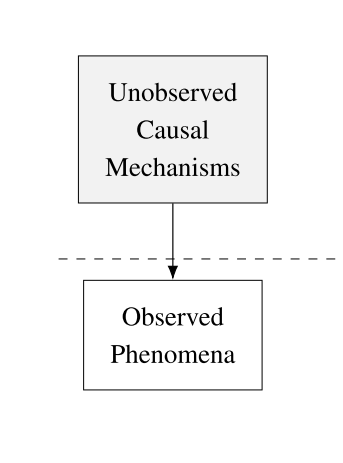
\includegraphics{scm_unobserved.png}
				}
			}
		\vspace{0.1cm}%
		\raggedleft \footnotesize \emph{Taken from \citep[p. 6]{BarenboimEtal2020}}
		\end{column}%
	\end{columns}	
\note[itemize]{
	\item{Reality is a garden of forking paths, we only see one potential outcome of many}
	\item{We cannot observe all potential outcomes for every individual}
}
\end{frame}


\begin{frame}{Simpson's Paradox}
	\begin{columns}[T]
		\begin{column}{0.58\linewidth}
		\only<1>{
				\centering
			\sffamily
			\begin{tabular}{cc|c}
				\multicolumn{3}{c}{Believe the Election Was Stolen} \\
				\multicolumn{3}{c}{} \\
				& & \thead[t]{Total} \\
				\cline{2-3}
				\multirow{3}{*}{\textbf{Misinfo}} & 
				Yes & \makecell[t]{47\% ($\frac{582}{1240}$)} \\
				& No &  \textcolor{blue}{\makecell[t]{60\% ($\frac{456}{760}$)}} \\
				\cline{2-3}
				&  & \makecell[t]{$\scriptstyle{\mathbb{E}[Y|T]}$} \\
			\end{tabular}
		}
		\only<2>{
			\centering
			\sffamily
			\begin{tabular}{cc|cc|c}
				\multicolumn{5}{c}{Believe the Election Was Stolen} \\
				\multicolumn{5}{c}{} \\
				& & \thead[t]{D} & \thead[t]{R} & \thead[t]{Total} \\
				\cline{2-5}
				\multirow{3}{*}{\textbf{Misinfo}}
				& Yes & \textcolor{blue}{\makecell[t]{30\% ($\tfrac{240}{800}$)}} & \textcolor{blue}{\makecell[t]{78\% ($\tfrac{342}{440}$)}} &\makecell[t]{47\% ($\frac{582}{1240}$)} \\
				& No & \makecell[t]{11\% ($\tfrac{16}{150}$)} & \makecell[t]{72\% ($\tfrac{440}{610}$)} & \textcolor{blue}{\makecell[t]{60\%   ($\frac{456}{760}$)}} \\
				\cline{2-5}
				&  & \makecell[t]{${\scriptstyle\mathbb{E}[Y|T,C=D]}$} & \makecell[t]{${\scriptstyle\mathbb{E}[Y|T,C=R]}$} & \makecell[t]{${\scriptstyle\mathbb{E}[Y|T]}$} \\
				
			\end{tabular}
		}
		\only<3->{
			\centering
			\sffamily
			\begin{tabular}{cc|cc|c}
				\multicolumn{5}{c}{Believe the Election Was Stolen} \\
				\multicolumn{5}{c}{} \\
				& & \thead[t]{D} & \thead[t]{R} & \thead[t]{Total} \\
				\cline{2-5}
				\multirow{3}{*}{\textbf{Misinfo}}
				& Yes & \textcolor{blue}{\makecell[t]{30\% ($\tfrac{240}{800}$)}} & \textcolor{blue}{\makecell[t]{78\% ($\tfrac{342}{440}$)}} &\makecell[t]{47\% ($\frac{582}{1240}$)} \\
				& No & \makecell[t]{11\% ($\tfrac{16}{150}$)} & \makecell[t]{72\% ($\tfrac{440}{610}$)} & \textcolor{blue}{\makecell[t]{60\%   ($\frac{456}{760}$)}} \\
				\cline{2-5}
				&  & \makecell[t]{${\scriptstyle\mathbb{E}[Y|T,C=D]}$} & \makecell[t]{${\scriptstyle\mathbb{E}[Y|T,C=R]}$} & \makecell[t]{${\scriptstyle\mathbb{E}[Y|T]}$} \\
				\multicolumn{5}{c}{} \\
				\multicolumn{5}{c}{
					$\begin{aligned}
						{\scriptstyle\mathbb{E}[Y|T=1] - \mathbb{E}[Y|T=0]} &{\scriptstyle= -0.13} \\
						{\scriptstyle\mathbb{E}[Y|T=1,C] - \mathbb{E}[Y|T=0,C]} &{\scriptstyle= 0.12}
					\end{aligned}$	
				} \\
%				\multicolumn{5}{c}{${}$} \\
				\multicolumn{5}{c}{} \\
				\multicolumn{5}{c}{\textbf{What is the effect of misinformation?}} 
			\end{tabular}
		}	
		\end{column}
		\hfill%
		\begin{column}{0.4\linewidth}
		\only<1>{
			\begin{wideitemize}
				\item Social media data on user engagement
				\item Consumers of misinformation are \textit{less} likely to believe the election was stolen
				\item Hmm... what is happening?
			\end{wideitemize}
		}
		\only<2->{
			\begin{wideitemize}
				\item When we group by party, the effect of misinformation flips
				\item[] $\underbrace{\textcolor{red}{\frac{800}{1240}}(0.3)}_{\text{\textcolor{red}{upweight}}} + \frac{440}{1240}(0.78) = 0.47$
				\item[] $\frac{150}{760}(0.11) + \underbrace{\textcolor{red}{\frac{610}{760}}(0.73)}_{\text{\textcolor{red}{upweight}}} = 0.60$
			\end{wideitemize}
		}	
		\end{column}
	\end{columns}
\note[itemize]{
	\item{We are studying the effect of misinformation on beliefs about the election}
	\item{Group by party, we see 800 out of 1240 people in sample who were exposed to misinformation were Democrats vs 440 Reps, so the 30\% is up-weighted}
	\item{Among non-exposed, far more Reps than Dems, so the 72\$ is up-weighted}
	\item{Which ATE is correct? Why and how do you know? Is the sample bad? How do you know? Where's the evidence? Everything is based on (plausible) assumptions (grounded prior knowledge).}
	\item{Once we wipe the fog from our glasses, all assumptions---about sample size or otherwise---are rooted in a causal structure, as we'll see. }
}
\end{frame}



\begin{frame}{The Ladder of Causation}
		\footnotesize
		\begin{tabularx}{\textwidth}{l lllll}
			\toprule
			& \thead[tl]{Layer \\ (Symbolic)} & \thead[tl]{Typical \\ Activity} & \thead[tl]{Typical \\ Question} & \thead[tl]{Example} & \thead[tl]{Statistics} \\
			\midrule
			\onslide<2->{
			$\mathcal{L}_1$ & \makecell[tl]{Associational \\ $P(y|x)$} & Seeing & \makecell[tl]{What is?\\How would seeing\\$X$ change my belief\\in $Y$?} & \makecell[tl]{What does a speech\\tell us about a\\politician's ideology?} & \makecell[tl]{Regression /\\Model fitting /\\MLE}
		}\\
		\onslide<3->{
			$\mathcal{L}_2$ & \makecell[tl]{Interventional \\ $P(y|do(x),c)$} & Doing & \makecell[tl]{What if?\\What if I do $X$?} & \makecell[tl]{What if we tax\\ carbon, will GHG\\emissions lower?} & \makecell[tl]{Experiment /\\Natural\\ Experiment /\\Adjustment}
		}\\
		\onslide<4->{
			$\mathcal{L}_3$ & \makecell[tl]{Counterfactual \\ $P(y_x|x^\prime,y^\prime)$} & Imagining & \makecell[tl]{Why?\\What if I had acted\\differently?} & \makecell[tl]{Was it the Russians\\that caused Trump\\to win?} & \makecell{\\(Adjustment)}
		}\\
		\midrule
		\multicolumn{6}{r}{\footnotesize Based on table from \citep[p. 8]{BarenboimEtal2020}} \\
		\bottomrule
			
		\end{tabularx}
\end{frame}

\begin{frame}{The Problem of Causal Inference}
	\begin{columns}[c] % align columns
		\begin{column}{.58\textwidth}
			\begin{wideitemize}
				\item<1-> The layers of the causal hierarchy are nested
				\item<2-> \emph{Generally impossible} to draw higher-layer inferences with only lower-layer information \citep{BarenboimEtal2020}
				\item<3-> Q: So what "information" allows us to move up the ladder?
				\item<4-> A: \emph{\textcolor{blue}{Causal assumptions}}
			\end{wideitemize}
		\end{column}
		\hfill%
		\begin{column}{.38\textwidth}
			\makebox[\linewidth][c]{
				\resizebox{\linewidth}{!}{
					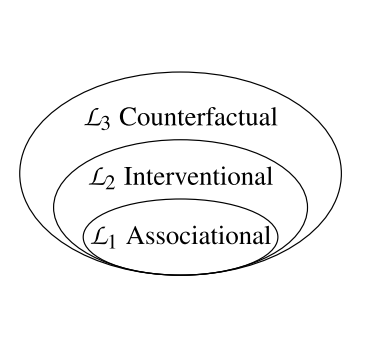
\includegraphics{scm_layers.png}
				}
			}
			\vspace{0.5cm}%
			\raggedleft \footnotesize \emph{Taken from \citep[p. 6]{BarenboimEtal2020}}
		\end{column}%
	\end{columns}
\note[itemize]{
	\item{What do we mean by "causal assumptions"?}
	\item{Where do "causal assumptions" come from?}
}
\end{frame}



\begin{frame}{The Problem of Causal Inference}
\begin{columns}[T] % align columns
\begin{column}{.5\textwidth}
\only<1>{
	\begin{center}
		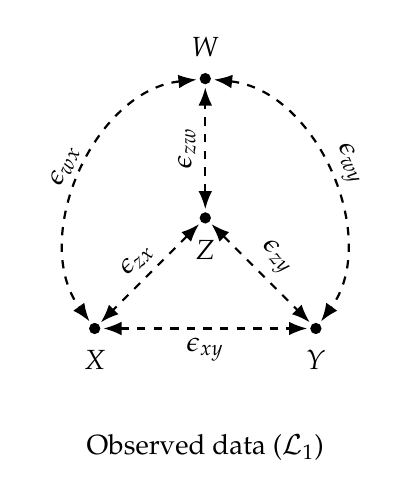
\begin{tikzpicture}[node distance =1.25 cm and 1.25 cm]
			% Title
			\node at (0, -3) {Observed data ($\mathcal{L}_1$)};
			
			\node (z) [label = below:$Z$, point];
			\node (w) [above = of z,yshift=0.3cm, label = above:$W$, point];
			\node (x) [label = below:$X$, below left = of z, point];
			\node (y) [label = below:$Y$, point, below right = of z];
			
			\path[bidirected] (z) edge node[above, el] {$\epsilon_{zy}$} (y);
			\path[bidirected] (z) edge node[above, el] {$\epsilon_{zx}$} (x);
			\path[bidirected] (z) edge node[above, el] {$\epsilon_{zw}$} (w);
			\path[bidirected] (w) edge[bend left= 60] node[above, el] {$\epsilon_{wy}$} (y);
			\path[bidirected] (w) edge[bend right=60] node[above, el] {$\epsilon_{wx}$} (x);
			\path[bidirected] (x) edge node[below, el] {$\epsilon_{xy}$} (y);
			
		\end{tikzpicture}
	\end{center}
}
\only<2>{
	\begin{center}
		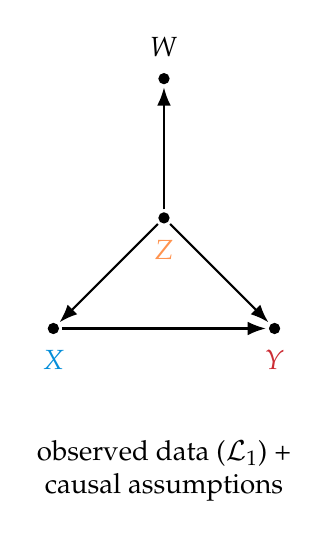
\begin{tikzpicture}[node distance =1.25 cm and 1.25 cm]
			% Title
			\node at (0, -3.5) {observed data ($\mathcal{L}_1$) +\\causal assumptions};
			
			\node (z) [label = below:\textcolor{orange}{$Z$}, point];
			\node (w) [above = of z,yshift=0.3cm, label = above:$W$, point];
			\node (x) [label = below:\textcolor{blue}{$X$}, below left = of z, point];
			\node (y) [label = below:\textcolor{red}{$Y$}, point, below right = of z];
			
			\path (z) edge node[above, el] {} (w);
			\path (z) edge node[above, el] {} (x);
			\path (z) edge node[above, el] {} (y);
			\path (x) edge node[below] {} (y);
			
		\end{tikzpicture}
	\end{center}
}
\only<3>{
		\begin{center}
		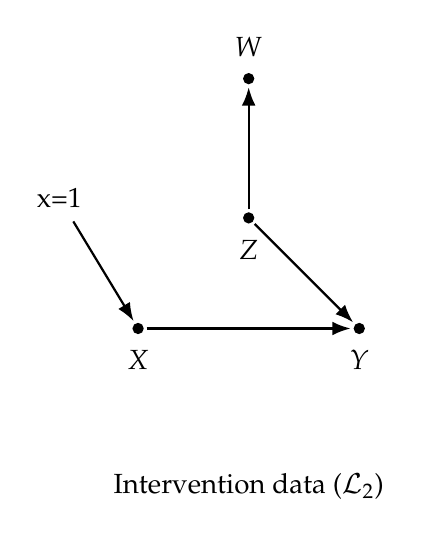
\begin{tikzpicture}[node distance =1.25 cm and 1.25 cm]
			% Title
			\node at (0, -3.5) {Intervention data ($\mathcal{L}_2$)};
			
			\node (z) [label = below:$Z$, point];
			\node (w) [above = of z,yshift=0.3cm, label = above:$W$, point];
			\node (x) [label = below:$X$, below left = of z, point];
			\node (y) [label = below:$Y$, point, below right = of z];
			\node (x_int) [above = of x, xshift=-1cm] {x=1};
			
			\path (z) edge node[above, el] {} (w);
			\path (z) edge node[above, el] {} (y);
			\path (x) edge node[below] {} (y);
			\path (x_int) edge node[below] {} (x);
			
		\end{tikzpicture}
	\end{center}
}
\only<4>{
	\begin{center}
		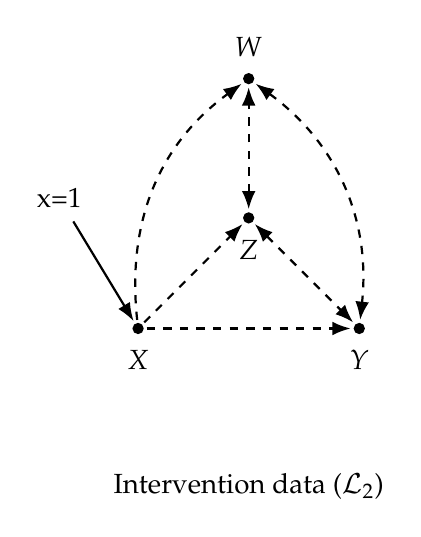
\begin{tikzpicture}[node distance =1.25 cm and 1.25 cm]
			% Title
			\node at (0, -3.5) {Intervention data ($\mathcal{L}_2$)};
			
			\node (z) [label = below:$Z$, point];
			\node (w) [above = of z,yshift=0.3cm, label = above:$W$, point];
			\node (x) [label = below:$X$, below left = of z, point];
			\node (y) [label = below:$Y$, point, below right = of z];
			\node (x_int) [above = of x, xshift=-1cm] {x=1};

			\path (x_int) edge node[below] {} (x);
			\path[latent] (x) edge node[above, el] {} (z);
			\path[latent] (x) edge[bend left=30] node[above, el] {} (w);
			\path[latent] (x) edge node[below, el] {} (y);
			\path[bidirected] (z) edge node[above, el] {} (y);
			\path[bidirected] (z) edge node[above, el] {} (w);
			\path[bidirected] (w) edge[bend left= 30] node[above, el] {} (y);
			
		\end{tikzpicture}
	\end{center}
}
\end{column}%
\hfill%
\begin{column}{.48\textwidth}
\only<1>{
  \begin{wideitemize}
  	\item At $\mathcal{L}_1$ we have a variable "salad"
  	\item In terms of probability, all we know is $P(X,Y,Z,W)$
  	\item Everything \emph{\textcolor{blue}{could be}} related to everything else
  	\item Best we can do is estimate associations (correlations)
  \end{wideitemize}
}
\only<2>{
	\begin{wideitemize}
		\item With knowledge + additional evidence, we \emph{\textcolor{blue}{assume}} away some paths
		\item Arrows imply conditional dependencies: 
		\begin{itemize}
			\item[$\implies$] $P(Y|Z,X)P(X,W|Z)P(Z)$
		\end{itemize}
		\item Still \emph{no intervention}, observed effect of \textcolor{blue}{$X$} on \textcolor{red}{$Y$} depends on \textcolor{orange}{$Z$}
	\end{wideitemize}
}
\only<3>{
	\begin{wideitemize}
		\item We set the value of $X$:
		\begin{itemize}
			\item[] $do(x=1)$
		\end{itemize}
	\end{wideitemize}
}
\only<4>{
	\begin{wideitemize}
		\item We set the value of $X$:
		\begin{itemize}
			\item[] $do(x=1)$
		\end{itemize}
		\item Causal assumptions rendered moot
		\item If $X$ influences $Y$, then a change in $X$ will appear as a change in $Y$
		\item[] $\mathbb{E}[Y|X=x_1]-\mathbb{E}[Y|X=x_0] \neq 0$
	\end{wideitemize}
}
\end{column}%
\end{columns}
\note[itemize]{
	\item{Explain DAG, nodes are variables, dashed edges represent potential relationships, arrows indicate direction of effect.}
	\item{\textbf{Ask audience member what they study}}
	\item{Imagine R dataframe with these variables, show it to your grandma or child. Does it mean anything to them? Let them play with some descriptive plots, can they tell you anything about direction of effects?}
	\item{Causal assumptions are represented by the absence of relationships (edges)}
	\item{Assuming NO relationship stricter than the contrary}
	\item{Intervening frees of of causal assumptions because we know value of X is independent (a la randomization)}
	\item{At $\mathcal{L}_3$ we observe some intervention, and want to know what would have happened had we altered the intervention or possibily some other variable in the system.}
}
\end{frame}


\begin{frame}{Simpson's Paradox Revisited}
	\begin{columns}[T]
	\begin{column}{0.58\linewidth}
		\only<1>{
			\begin{wideitemize}
				\item What is the effect of misinformation on the belief that the 2020 election was fraudulent?
				\item[]\begin{itemize}
					\item[]
					\item[] $\begin{aligned}
						\mathbb{E}[Y|T=1] & -\mathbb{E}[Y|T=0]= -0.13 \\
						&\text{or} \\
						\mathbb{E}[Y|T=1,C] & -\mathbb{E}[Y|T=0,C]=0.12
					\end{aligned}$
				\end{itemize}
			\end{wideitemize}
		}
		\only<2-3>{
			\begin{wideitemize}
				\item What is the effect of misinformation on the belief that the 2020 election was fraudulent?
				\item[]\begin{itemize}
					\item[]
					\item[] $\begin{aligned}
						\mathbb{E}[Y|T=1] & -\mathbb{E}[Y|T=0]= -0.13 \\
						&\text{or} \\
						\mathbb{E}[Y|T=1,C] & -\mathbb{E}[Y|T=0,C]=0.12
					\end{aligned}$
				\end{itemize}
				\item It depends on your causal assumptions
			\end{wideitemize}
		}
		\only<4>{
			\begin{wideitemize}
			\item What is the effect of misinformation on the belief that the 2020 election was fraudulent?
			\item[]\begin{itemize}
				\item[]
				\item[] $\begin{aligned}
					\mathbb{E}[Y|T=1] & -\mathbb{E}[Y|T=0]= -0.13 \\
					&\text{or} \\
					\Scale[1.2]{\textcolor{blue}{\mathbb{E}[Y|T=1,\textcolor{red}{C}]}} & \Scale[1.2]{\textcolor{blue}{-\mathbb{E}[Y|T=0,\textcolor{red}{C}]=0.12}}
				\end{aligned}$
			\end{itemize}
			\item It depends on your causal assumptions
		\end{wideitemize}
		}
		\only<5>{
			\begin{wideitemize}
			\item What is the effect of misinformation on the belief that the 2020 election was fraudulent?
			\item[]\begin{itemize}
				\item[]
				\item[] $\begin{aligned}
					\Scale[1.2]{\textcolor{blue}{\mathbb{E}[Y|T=1]}} & \Scale[1.2]{\textcolor{blue}{-\mathbb{E}[Y|T=0]= -0.13}} \\
					&\text{or} \\
					\mathbb{E}[Y|T=1,C] & -\mathbb{E}[Y|T=0,C]= 0.12
				\end{aligned}$
			\end{itemize}
			\item It depends on your causal assumptions
		\end{wideitemize}
		}
	\end{column}
		\hfill %
	\begin{column}{0.4\linewidth}
		\only<3>{
			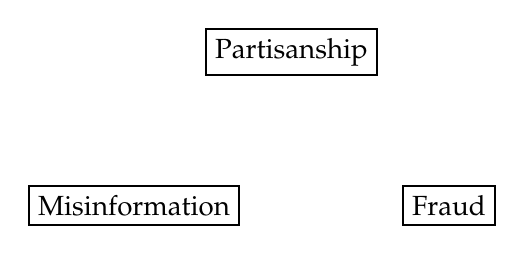
\begin{tikzpicture}[node distance =0.5 cm and 0.5 cm]
				% Title
				
				\node[state, rectangle] (1) at (0, 0) {Partisanship};
				\node[state, rectangle] (2) at (-2, -2) {Misinformation};
				\node[state, rectangle] (3) at (2, -2) {Fraud};
			\end{tikzpicture}
		}
		\only<4>{
			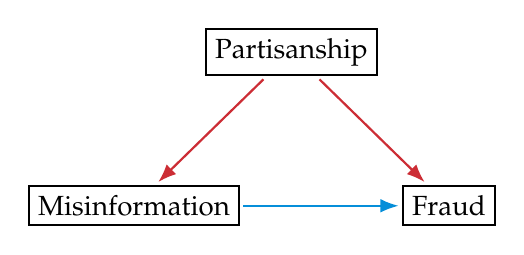
\begin{tikzpicture}[node distance =0.5 cm and 0.5 cm]
				% Title
				
				\node[state, rectangle] (1) at (0, 0) {Partisanship};
				\node[state, rectangle] (2) at (-2, -2) {Misinformation};
				\node[state, rectangle] (3) at (2, -2) {Fraud};
				
				\path[red] (1) edge node[above, el] {} (2);
				\path[red] (1) edge node[above, el] {} (3);
				\path[blue] (2) edge node[above, el] {} (3);
				
			\end{tikzpicture}
		}
		\only<5>{
			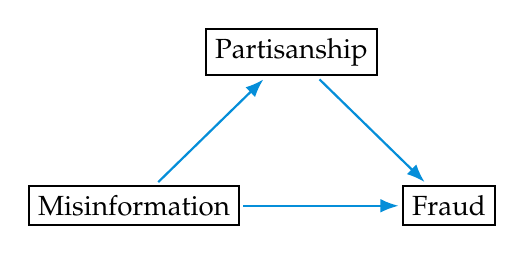
\begin{tikzpicture}[node distance =0.5 cm and 0.5 cm]
				% Title
				
				\node[state, rectangle] (1) at (0, 0) {Partisanship};
				\node[state, rectangle] (2) at (-2, -2) {Misinformation};
				\node[state, rectangle] (3) at (2, -2) {Fraud};
				
				\path[blue] (2) edge node[above, el] {} (1);
				\path[blue] (1) edge node[above, el] {} (3);
				\path[blue] (2) edge node[above, el] {} (3);
				
			\end{tikzpicture}
		}
	\end{column}
	\end{columns}
\note[itemize]{
	\item{Does partisanship influence consumption of misinformation \textit{and} belief in stop the steal? Very plausible, lot of evidence suggests this is the case}
	\item{However, maybe you think exposure to/consumption of misinfo influences partianship. E.g. friends who used to be progressive, slowly become Republican after years of consuming conspiratorial content on the internet.}
	\item{In scenario two, by comparing effects, we see that direct effect of misinformation is positive, but total effect is negative which suggests that indirect channel through partisanship is negative. Maybe, for average voter, exposure to misinfo turns then \textit{away} from the Republicans because of content and leads them to become more left-leaning.}
	\item{Both are plausible, require further validation of causal assumptions}
}

\end{frame}


\begin{frame}{The Problem of Causal Inference}
	\begin{adjustwidth*}{1em}{1em}
		\begin{flushleft}
			\Large "The central question in the analysis of causal effects is the question of \emph{\textcolor{red}{identification}}: can the controlled (post-intervention) distribution, $P(Y=y|do(x))$, be estimated from data governed by the pre-intervention distribution $P(X,Y,Z,W)$?"
		\end{flushleft}
		\begin{flushright}
			- \large \citeauthor{Pearl2009} (\citeyear{Pearl2009}, p. 108)
		\end{flushright}
	\end{adjustwidth*}
\end{frame}

\begin{frame}{The Problem of Causal Inference}
	\begin{wideitemize}
		\item<1-> Thus, the key to causal inference is achieving identification
		\item<2-> In experiments, identification is built-in since \textit{we} control the treatment
		\item<3-> In observational data, identification is tougher and, sometimes, \textit{unachievable} 
		\item<4-> So why not only do experiments?
	\end{wideitemize}
\end{frame}

\section{Experiments vs the World}
\begin{transitionframe}
	\begin{center}
		{ \Huge \textcolor{blue}{Experiments vs the World}}
	\end{center}
\end{transitionframe}

\begin{frame}{Experiments: Pros and Cons}
	\begin{columns}[T] %
		\begin{column}{.45\textwidth}
			\Large Pros
			\normalsize
			\begin{wideitemize}
				\item<1-> Identification guaranteed
				\item[]<2-> $\implies$\textcolor{blue}{Internal validity}
				\item<3-> Greater control over intervention
			\end{wideitemize}
		\end{column}
		\hfill%
		\begin{column}{.45\textwidth}
			\Large Cons
			\normalsize
			\begin{wideitemize}
				\item<4-> limits, limits, limits...
				\begin{itemize}
					\item<5-> ethical
					\item<6-> physical
					\item<7-> temporal
					\item<8-> external validity / transportability
				\end{itemize} 
				\item<9-> Causal mechanism still an assumption
			\end{wideitemize}
		\end{column}
	\end{columns}
\note[itemize]{
	\item{Control over who you want to assign treatments to and how}
	\item{e.g. different types of sampling}
	\item{Can design the experiment to directly assess research question of interest}
	\item{Ethical example cannot start a war}
	\item{Physical example limited to phenomena you can examine in a lab or survey}
	\item{Temporal example many causal chains stretch over long time scales, longitudinal studies expensive}
	\item{Transportability highly unlikely that the sample you achieved is perfectly random and free of selection bias, effects unbiased within the sample, but not population of interest}
}
\end{frame}


\begin{frame}{Observational Studies: Pros and Cons}
	\begin{columns}[T] %
		\begin{column}{.45\textwidth}
			\Large Pros
			\normalsize
			\begin{wideitemize}
				\item<1-> Can study phenomena of interest
				\item<2-> ...in the population of interest
				\item[]<3-> $\implies$\textcolor{blue}{external validity}
			\end{wideitemize}
		\end{column}
		\hfill%
		\begin{column}{.45\textwidth}
			\Large Cons
			\normalsize
			\begin{wideitemize}
				\item<4-> Identification challenged by
				\begin{itemize}
					\item<5-> selection bias
					\item<6-> non-random treatment
					\item<7-> data limitations
				\end{itemize} 
				\item<9-> Identification may be impossible without more data or experiment
			\end{wideitemize}
		\end{column}
	\end{columns}
\end{frame}

\section{PO vs SCM}
\begin{transitionframe}
	\begin{center}
		{ \Huge \textcolor{blue}{Potential Outcomes\\vs\\Structural Causal Models}}
	\end{center}
\end{transitionframe}

\begin{frame}{Potential Outcomes}
	\begin{columns}[c]
		\begin{column}{0.58\textwidth}
			\begin{wideitemize}
				\item Associated with \citet{Neyman1923} and \citet{Rubin1974}
				\item Widely adopted in social sciences and medicine
				\item Randomized experiment serve as its ruling paradigm
			\end{wideitemize}
		\end{column}
		\hfill%
		\begin{column}{0.4\textwidth}
			\makebox[\linewidth][c]{
				\resizebox{0.5\linewidth}{!}{
					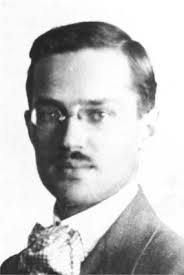
\includegraphics{neyman.jpg}
				}
				\resizebox{0.5\linewidth}{!}{
					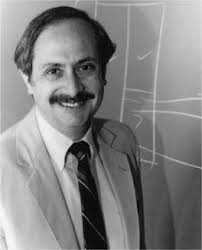
\includegraphics{rubin.jpeg}
				}
			}
		\end{column}
	\end{columns}
\end{frame}

\begin{frame}{Potential Outcomes}
	\begin{wideitemize}
		\item<1-> Object of analysis is a unit-based response variable
		\begin{itemize}
			\item patients
			\item survey respondents
			\item cities
		\end{itemize}
		\item<2-> Comparison between factual and \textcolor{blue}{counterfactual} for each unit $i$
		\item<3-> Denoted $Y_i(T_i)$
		\item<4-> "The value outcome $Y$ would obtain in experimental unit $i$ had treatment $T_i$ been $t$" 
	\end{wideitemize}
\end{frame}
	
\begin{frame}{Potential Outcomes}
	\begin{columns}[c]
		\begin{column}{0.45\textwidth}
			\begin{wideitemize}
				\item Units: $i = 1,\ldots,N$
				\item "Treatment": 
				\begin{itemize}
					\item $T_i=1$ if treated
					\item $T_i=0$ otherwise
				\end{itemize}
				\item \textit{Observed} outcome: $Y_i$
				\item Pre-treatment covariates: $X_i$
				\item Potential outcomes: $Y_i(1)$ and $Y_i(0)$
			\end{wideitemize}
		\end{column}%
		\hfill%
		\begin{column}{0.53\textwidth}
			\footnotesize
			\begin{tabular}{cccccc}
				\toprule
				\thead[tc]{Voters} & \thead[tc]{Contact} &\multicolumn{2}{c}{\thead{Turnout}} & \thead[tc]{Age} & \thead[tc]{Party ID} \\
				$i$ & $T_i$ & $Y_i(1)$ & $Y_i(0)$ & $X_i$ & $X_i$ \\
				\midrule
				1 & 1 & 1 & \textcolor{blue}{?} & 19 & D \\
				2 & 0 & \textcolor{blue}{?} & 0 & 45 & D \\
				3 & 0 & \textcolor{blue}{?} & 1 & 36 & R \\
				$\vdots$ & $\vdots$ & $\vdots$ & $\vdots$ & $\vdots$ & $\vdots$\\
				N & 1 & 0 & \textcolor{blue}{?} &  71 & R \\
				\bottomrule
			\end{tabular}
		\end{column}
	\end{columns}
\note[itemize]{
	\item{For each voter, we only observed one outcome}
	\item{We cannot simultaneously observe two universes, one where individual i is given treatment and one where not, then compare}
}
\end{frame}

\begin{frame}{Potential Outcomes Assumptions}
	\begin{columns}[c]
		\begin{column}{0.48\textwidth}
			Core Assumptions
			\begin{wideitemize}
				\item[1.]<1-> \textcolor{red}{No simultaneity}
				\item[2.]<2-> \textcolor{red}{No interference} between units
				\item[3.]<3-> \textcolor{red}{Same version} of treatment
			\end{wideitemize}
		\end{column}
		\hfill %
		\begin{column}{0.5\textwidth}
		\only<1>{
				\begin{center}
				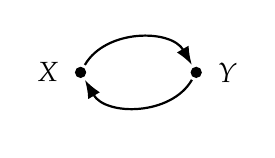
\begin{tikzpicture}[node distance =1.25 cm and 1.25 cm]	
%					\node (z) [label = below:$Z$, point];
%					\node (w) [above = of z,yshift=0.3cm, label = above:$W$, point];
					\node (x) [label = left:$X$, xshift=-1cm, point];
					\node (y) [label = right:$Y$, point, right = of x];
%					\node (x_int) [above = of x, xshift=-1cm] {x=1};
					
%					\path (x_int) edge node[below] {} (x);
%					\path[latent] (x) edge node[above, el] {} (z);
%					\path[latent] (x) edge[bend left=30] node[above, el] {} (w);
					\path (x) edge[bend left = 60] node[below] {} (y);
					\path (y) edge[bend left = 60] node[below] {} (x);
%					\path[bidirected] (z) edge node[above, el] {} (y);
%					\path[bidirected] (z) edge node[above, el] {} (w);
%					\path[bidirected] (w) edge[bend left= 30] node[above, el] {} (y);
					
				\end{tikzpicture}
			\end{center}
		}
		\only<2>{
			\begin{center}
				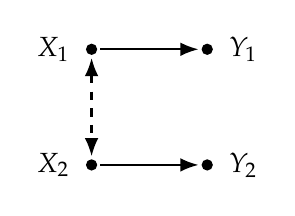
\begin{tikzpicture}[node distance =1.25 cm and 1.25 cm]	

					\node (x1) [label = left:$X_1$, xshift=-1cm, point];
					\node (y1) [label = right:$Y_1$, point, right = of x1];
					\node (x2) [label = left:$X_2$, below = of x1, point];
					\node (y2) [label = right:$Y_2$, point, right = of x2];

					\path (x1) edge node[below] {} (y1);
					\path[bidirected] (x1) edge node[below] {} (x2);
					\path (x2) edge node[below] {} (y2);
				\end{tikzpicture}
			\end{center}
		}
		\only<4->{
			
			\begin{wideitemize}
				\item Stable Unit Treatment Value Assumption (SUTVA)
				\item Potential violations:
				\begin{itemize}
					\item feedback effects
					\item spill-over effects
					\item different treatment administration
				\end{itemize}
				\item Observed outcome is random because \textcolor{blue}{treatment is random}
				\item Multi-valued treatment: more potential outcomes for each unit
			\end{wideitemize}	
	}
		\end{column}
	\end{columns}
\end{frame}

\begin{frame}{Potential Outcomes Assumptions}
	\begin{columns}[T] % align columns
		\begin{column}{.5\textwidth}
			\only<1>{
				\begin{center}
					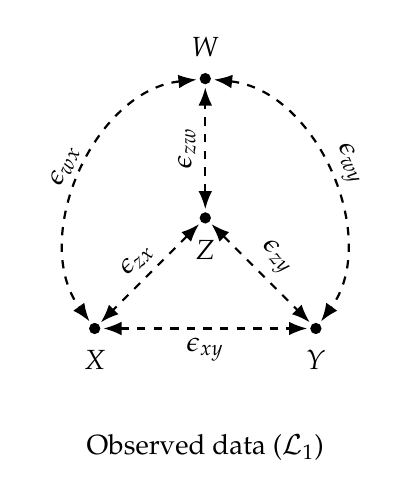
\begin{tikzpicture}[node distance =1.25 cm and 1.25 cm]
						% Title
						\node at (0, -3) {Observed data ($\mathcal{L}_1$)};
						
						\node (z) [label = below:$Z$, point];
						\node (w) [above = of z,yshift=0.3cm, label = above:$W$, point];
						\node (x) [label = below:$X$, below left = of z, point];
						\node (y) [label = below:$Y$, point, below right = of z];
						
						\path[bidirected] (z) edge node[above, el] {$\epsilon_{zy}$} (y);
						\path[bidirected] (z) edge node[above, el] {$\epsilon_{zx}$} (x);
						\path[bidirected] (z) edge node[above, el] {$\epsilon_{zw}$} (w);
						\path[bidirected] (w) edge[bend left= 60] node[above, el] {$\epsilon_{wy}$} (y);
						\path[bidirected] (w) edge[bend right=60] node[above, el] {$\epsilon_{wx}$} (x);
						\path[bidirected] (x) edge node[below, el] {$\epsilon_{xy}$} (y);
						
					\end{tikzpicture}
				\end{center}
			}
		\only<2->{
			\begin{center}
				\begin{tikzpicture}[node distance =1.25 cm and 1.25 cm]
					% Title
					\node at (0, -3.5) {Intervention data ($\mathcal{L}_2$)};
					
					\node (x) [label = below:$X$, xshift=-1cm, point];
					\node (y) [label = below:$Y$, point, right = of x];
					\node (x_int) [above = of x, xshift=-1cm] {x=1};
					
					\path (x_int) edge node[below] {} (x);
					\path[latent] (x) edge node[below, el] {} (y);
					
				\end{tikzpicture}
			\end{center}
		}
		\end{column}%
		\hfill%
		\begin{column}{.48\textwidth}
			Crux of PO is randomized treatment
			\begin{wideitemize}
				\item<1-> Causal mechanism too complex to rule out no omitted variable with certainty
				\item<2-> Looks for "as-if" random treatments or proxy treatments
				\item<2-> Allows you to \textcolor{orange}{ignore} possible confounders
			\end{wideitemize}
		\end{column}%
	\end{columns}
\end{frame}

\begin{frame}{Potential Outcomes Research Designs}
	\begin{wideitemize}
		\item Preferred research designs based on exogeneity assumption:
		\begin{itemize}
			\item Instrumental Variables (IV)
			\item Regression Discontinuity Design (RDD)
			\item Difference-in-Difference (DiD)
		\end{itemize}
		\item When we cannot find intervention data: matching
		\item \textcolor{red}{Criticisms:}
		\begin{itemize}
			\item exogeneity assumption almost always untestable
			\item finding guaranteed random treatments in the wild is extremely rare
			\item OR the randomized "treatment" doesn't quite align with the theory we want to test
		\end{itemize} 
	\end{wideitemize}
\end{frame}

\begin{frame}{Structural Causal Models}
	\begin{columns}[c]
		\begin{column}{0.58\textwidth}
			\begin{wideitemize}
				\item Associated with \citet{Pearl2000} but many predecessors and successors
				\item Emerged from computer science field, but builds on:
				\begin{itemize}
					\item structural equation models (SEM) \citep{Goldberger1973}
					\item potential outcomes
					\item probabilistic graphical models \citep{Lauritzen1996, SpirtesEtal2000}
				\end{itemize}
				\item The causal graph serves as ruling paradigm
				\item sometimes referred to as a "DAG" (directed acyclic graph)
			\end{wideitemize}
		\end{column}
		\hfill%
		\begin{column}{0.4\textwidth}
			\makebox[\linewidth][c]{
				\resizebox{0.5\linewidth}{!}{
					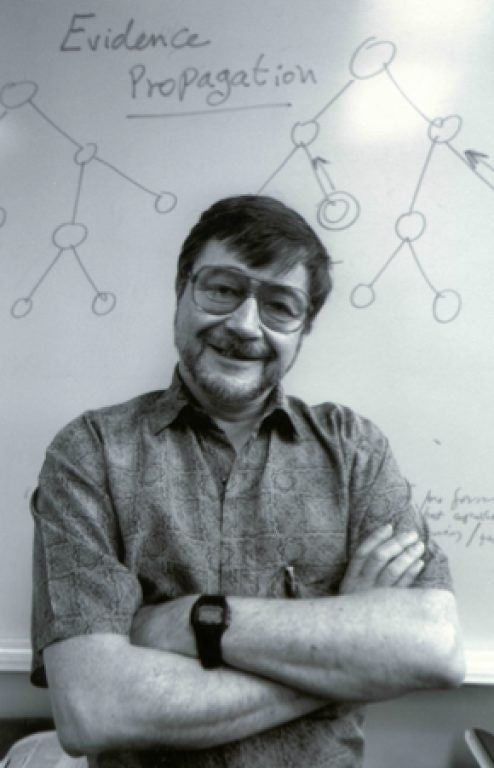
\includegraphics{pearl.jpg}
				}
			}
		\end{column}
	\end{columns}
\end{frame}

\begin{frame}{Structural Causal Models}
	\begin{wideitemize}
		\item<1-> Based on a directed graph that displays casual relationships between variables
		\item Models sometimes defined as ordered triples $\langle U, V, E \rangle$:
		\begin{itemize}
			\item Exogenous variables $U$
			\item Endogenous variables $V$
			\item Set of equations $E$ that defining relationships between $V$ 
		\end{itemize}
		\item<2-> The models are probabilistic and \textcolor{blue}{represent} a unique factorization of a joint probability distribution into \textcolor{blue}{conditional probabilities}
		\item<3-> Use \textcolor{blue}{\textit{do}-calculus} to achieve identification on observed data
	\end{wideitemize}
\end{frame}

\begin{frame}{SCM Assumptions}
	\begin{columns}[c]
		\begin{column}{0.38\textwidth}
			\only<1>{
				\begin{center}
					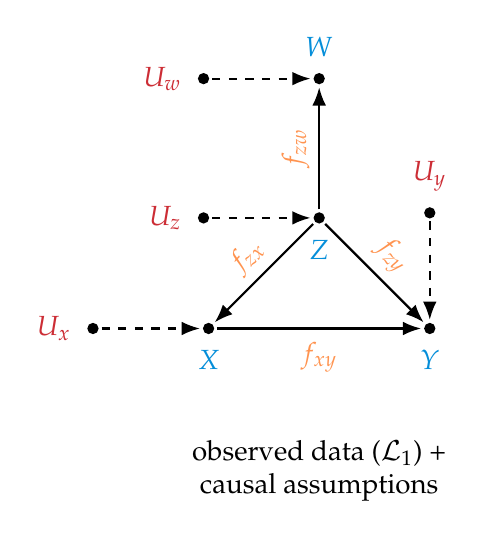
\begin{tikzpicture}[node distance =1.25 cm and 1.25 cm]
						% Title
						\node at (0, -3.5) {observed data ($\mathcal{L}_1$) +\\causal assumptions};
						
						\node (z) [label = below:\textcolor{blue}{$Z$}, point];
						\node (w) [above = of z,yshift=0.3cm, label = above:\textcolor{blue}{$W$}, point];
						\node (x) [label = below:\textcolor{blue}{$X$}, below left = of z, point];
						\node (y) [label = below:\textcolor{blue}{$Y$}, point, below right = of z];
						\node (ux) [label = left:\textcolor{red}{$U_x$}, point, left = of x];
						\node (uz) [label = left:\textcolor{red}{$U_z$}, point, left = of z];
						\node (uy) [label = above:\textcolor{red}{$U_y$}, point, above = of y];
						\node (uw) [label = left:\textcolor{red}{$U_w$}, point, left = of w];
						
						\path (z) edge node[above, el] {\textcolor{orange}{$f_{zw}$}} (w);
						\path (z) edge node[above, el] {\textcolor{orange}{$f_{zx}$}} (x);
						\path (z) edge node[above, el] {\textcolor{orange}{$f_{zy}$}} (y);
						\path (x) edge node[below] {\textcolor{orange}{$f_{xy}$}} (y);
						
						\path[latent] (ux) edge node[above, el] {} (x);
						\path[latent] (uz) edge  node[above, el] {} (z);
						\path[latent] (uy) edge node[below] {} (y);
						\path[latent] (uw) edge node[above, el] {} (w);
						
					\end{tikzpicture}
				\end{center}
			}
			\only<2->{
			\begin{center}
				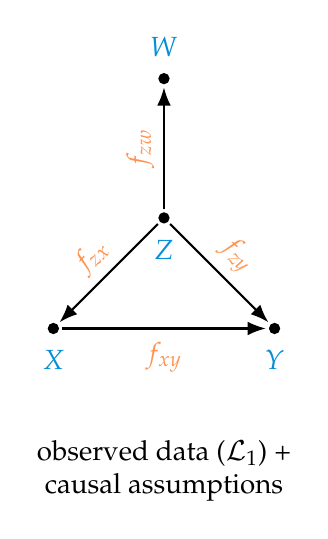
\begin{tikzpicture}[node distance =1.25 cm and 1.25 cm]
					% Title
					\node at (0, -3.5) {observed data ($\mathcal{L}_1$) +\\causal assumptions};
					
					\node (z) [label = below:\textcolor{blue}{$Z$}, point];
					\node (w) [above = of z,yshift=0.3cm, label = above:\textcolor{blue}{$W$}, point];
					\node (x) [label = below:\textcolor{blue}{$X$}, below left = of z, point];
					\node (y) [label = below:\textcolor{blue}{$Y$}, point, below right = of z];
					
					\path (z) edge node[above, el] {\textcolor{orange}{$f_{zw}$}} (w);
					\path (z) edge node[above, el] {\textcolor{orange}{$f_{zx}$}} (x);
					\path (z) edge node[above, el] {\textcolor{orange}{$f_{zy}$}} (y);
					\path (x) edge node[below] {\textcolor{orange}{$f_{xy}$}} (y);
					
				\end{tikzpicture}
			\end{center}
		}
		\end{column}%
		\hfill
		\begin{column}{0.6\textwidth}
			\begin{wideitemize}
				\item<1-> The notation seems scary, but we saw this before
				\begin{itemize}
					\item<2-> $U$ are independent of what happens within the system
					\item<2-> $V$ are dependent on system
					\item<3-> $E$ represents functional relationships
				\end{itemize}
				\item<4-> All assumptions are encoded into the graph itself
				\item<5-> Since the graph represents conditional probabilities, we can determine what variables to adjust for from it
				\item<6-> Theory$\implies$assumptions
			\end{wideitemize}
		\end{column}
	\end{columns}
\end{frame}

\begin{frame}{Model Elements}
	\begin{columns}[c]
		\begin{column}{0.5\textwidth}
		\only<1>{
			All DAGs are built from three fundamental relationships
		}	
		\only<2>{
			Chain
			\begin{wideitemize}
				\item Straight line connections with arrows pointing from cause to effect
				\item $B$ mediates effect of $A$ on $C$
			\end{wideitemize}
		}
		\only<3>{
			Fork
			\begin{wideitemize}
				\item One cause has multiple effects
				\item There exists spurious correlation between $A$ and $C$ due to $B$
				\item Eliminate by adjusting for $B$
			\end{wideitemize}	
		}
		\only<4>{
			Collider
			\begin{wideitemize}
				\item Multiple causes affect one outcome
				\item Conditioning on $B$ often induces a non-causal negative relationship between $A$ and $C$
				\item Collider bias, wherein $B$ explains away correlation between $A$ and $C$
			\end{wideitemize}
		}
		\end{column}%
		\hfill
		\begin{column}{0.48\textwidth}
		\only<2>{
			\begin{center}
				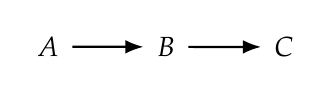
\begin{tikzpicture}[node distance =1.25 cm and 1.25 cm]	
					
					\node (a) at (-1.5, 0) {$A$};
					\node (b) at (0, 0) {$B$};
					\node (c) at (1.5, 0) {$C$};
					
					\path (a) edge (b);
					\path (b) edge (c);
					
				\end{tikzpicture}
			\end{center}
		}
		\only<3>{
			\begin{center}
				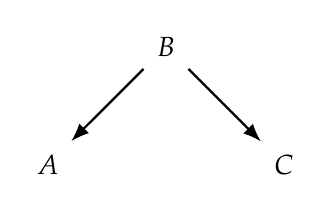
\begin{tikzpicture}[node distance =1.25 cm and 1.25 cm]	
					
					\node (a) at (-1.5, 0) {$A$};
					\node (b) at (0, 1.5) {$B$};
					\node (c) at (1.5, 0) {$C$};
					
					\path (b) edge (a);
					\path (b) edge (c);
					
				\end{tikzpicture}
			\end{center}	
		}
		\only<4>{
			\begin{center}
				\begin{tikzpicture}[node distance =1.25 cm and 1.25 cm]	
					
					\node (a) at (-1.5, 1.5) {$A$};
					\node (b) at (0, 0) {$B$};
					\node (c) at (1.5, 1.5) {$C$};
					
					\path (a) edge (b);
					\path (c) edge (b);
					
				\end{tikzpicture}
			\end{center}	
		}		
		\end{column}
	\end{columns}
\end{frame}

\begin{frame}{Identification with DAGS}
	Identification is achieved via \textit{do}-calculus
	\begin{columns}[c]
		\begin{column}{0.5\textwidth}
			\begin{wideitemize}
				\item Set of rules for determining a minimally-sufficient set of adjustment variables
				\item Examine all paths between treatment and outcome, control for confounders
				\item Not too complicated, but beyond scope of presentation
			\end{wideitemize}
		\end{column}
		\hfill
		\begin{column}{0.48\textwidth}
			\begin{center}
				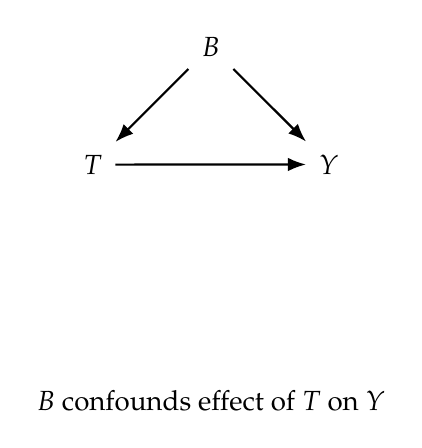
\begin{tikzpicture}[node distance =1.25 cm and 1.25 cm]	
					\node at (0, -3) {$B$ confounds effect of $T$ on $Y$};
					
					\node (a) at (-1.5, 0) {$T$};
					\node (b) at (0, 1.5) {$B$};
					\node (c) at (1.5, 0) {$Y$};
					
					\path (b) edge (a);
					\path (b) edge (c);
					\path (a) edge (c);
					
				\end{tikzpicture}
			\end{center}
		\end{column}
	\end{columns}
\end{frame}

\begin{frame}{SCM as a Language}
	\begin{wideitemize}
		\item SCMs represents a \textit{language} of causality
		\item All other approaches to causal inference can be encoded in a DAG (i.e. PO is subsumed by SCM)
		\item Can also be used to determine when and how to escape from \textcolor{orange}{selection bias}
		\item \textcolor{red}{Criticisms:}
		\begin{itemize}
			\item Encoding our theory into a DAG can be \textit{hard}
			\item Complex theory $\implies$ complex DAG
			\item[$\hookrightarrow$] DAGs can become overwhelming, fast
			\item do-calculus only guarantees identification if theory is correct
		\end{itemize}
		\item \href{www.dagitty.net}{Dagitty}: tool that performs do-calculus for you, has \texttt{R} package too
	\end{wideitemize}
\end{frame}
\note[itemize]{
	\item{Critique of assumption true in all models}
}

\section{Conclusion}
\begin{transitionframe}
	\begin{center}
		{ \Huge \textcolor{blue}{Conclusion}}
	\end{center}
\end{transitionframe}

\begin{frame}{Conclusion}
	\begin{wideitemize}
		\item Randomized experiments are considered a \colorbox{Goldenrod}{gold standard} for causal inference
		\item But they are \colorbox{Black}{\textcolor{White}{black boxes}}
		
		\item The key to causal inference on observational data is:
		\begin{itemize}
			\item make stronger assumptions about the relationships between variables
			\item Search for interventional $\mathcal{L}_2$ setups that match theory 
		\end{itemize}
		\item In SCM, we do the former and establish whether observational data is identified; if not, ask is it achievable and how?
		\item In PO, identifiability is guaranteed so long as we believe intervention is truly random
		\item Both require rigorous validation of assumptions
		\item Once identified, we can interpret $\beta$ as a causal effect 
	\end{wideitemize}
\end{frame}
\note[itemize]{
	\item{All the work goes into developing good identification strategies and validating that strategy}
	\item{Once you achieve identification, there's still a question of the "correct" functional form.}
}

% Uncomment slide for bibliography
\begin{frame}[allowframebreaks]{References}
	\printbibliography
\end{frame}



%\appendix

%\begin{frame}[label=appendix_start]{Almost done!}
%  \begin{wideitemize}
%  \item See, now we're in backup slide land
%  \item This is made useful by having links throughtout the talk
%  \item Here's a button, which is how I make links \hyperlink{appendix_end}{\beamergotobutton{Next slide}}
%  \end{wideitemize}
%\end{frame}
%
%\begin{frame}[label=appendix_end]{Use it to intimidate audiences!}
%  \begin{wideitemize}
%    \item[] Now you can make it clear you've done a shitload of work
%      \begin{itemize}
%      \item[]  without having to show everything! \hyperlink{appendix_start}{\beamergotobutton{Back}}
%      \end{itemize}
%    \item[] You label a frame with the \texttt{[label=name]} option, and then point a link to it
%    \item[] You can make an object a link using the \texttt{\textbackslash hyperlink\{label\}\{object\}} command
%  \end{wideitemize}
%\end{frame}


\end{document}